\newpage
\section{Durchführung}
\label{sec:Durchfuehrung}
\begin{figure}
    \centering
    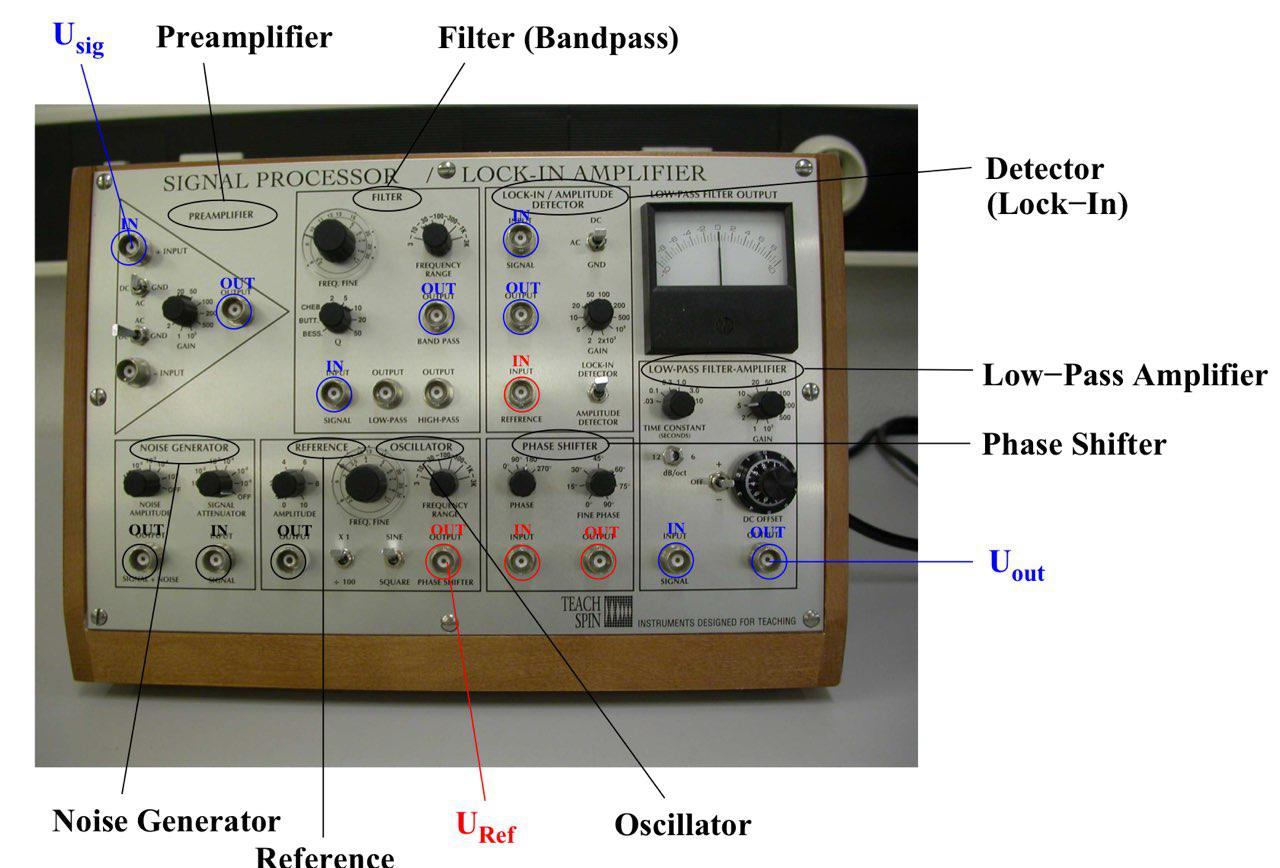
\includegraphics[width=0.5\textwidth]{bilder/aufbau.jpg}
    \caption{Lock-In-Verstärker,\cite[3]{Anleitung}}        
    \label{fig:aufbau}
\end{figure}


Es lassen sich alle Signalteile wie Vorverstärker, Filter, Phasenschieber, Funktionsgenerator, Rauschgenerator,
Tiefpass-Verstärker und ein Amplituden-/Lock-In-Detektor seperat bedienen.

\begin{enumerate}
\item Kennenlernen des Reference/Oscillator.\\ Dieser verfügt über zwei
Ausgänge (vgl. dazu Abb \ref{fig:aufbau}).
Beide Ausgänge werden an ein Oszilloskop angeschlossen und die Variationsmöglichkeiten
der Spannungsamplitude untersucht. 
\item Untersuchen von Phasenschieber und Tiefpass\\
Dafür wird die Schaltung aus Abb. \ref{fig:aufbau_schema2} verwendet.
Zunächst wird der Noise Generator überbrückt. Ein Nutzsignal von ca. $1kHz$ und $10mV$
wird mit einem Referenzsignal der gleichen Frequenz gemischt.\\
Untersucht wird dabei, das Verhalten beim ändern der Phase $\Phi$.
Dafür werden fünf verschieden Phasen eingestellt und das Ausgangssignal skizziert.
\begin{figure}[H]
    \centering
    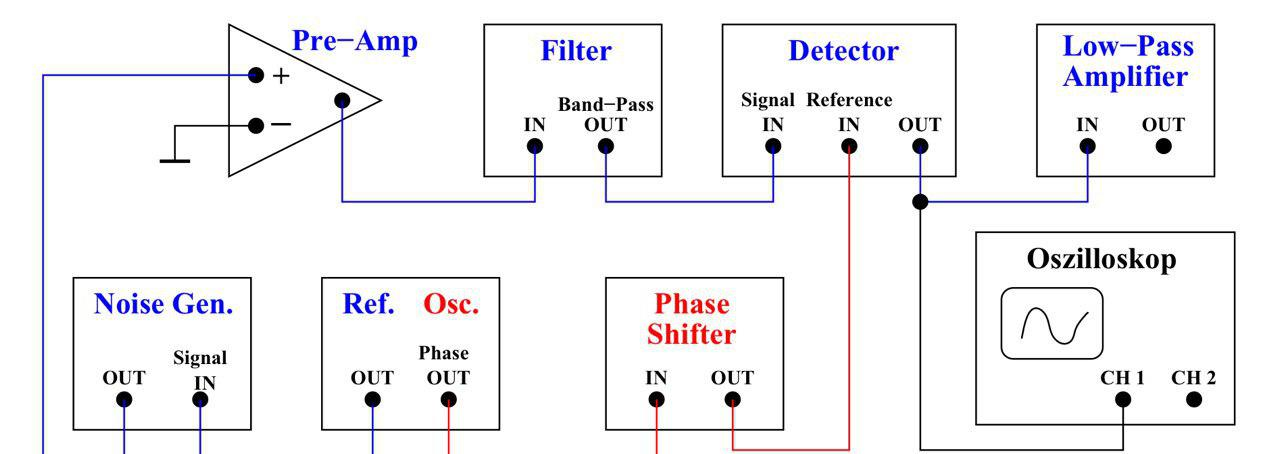
\includegraphics[width=0.7\textwidth]{bilder/aufbau_schema2.jpg}
    \caption{Schema Lock-In-Verstärker,\cite[4]{Anleitung}}
    \label{fig:aufbau_schema2}
\end{figure}
\item Im Anschluss wird das Ausgangssignal integriert und die Asugangspannung
in Abhängigkeit der Phasenverschiebung verglichen.
\item Nun wird der Noise Generator dazu geschaltet und ebenfalls
die Veränderung des Ausgangsignals für verschiedene Phasen $\Phi$ mit und ohne Tiefpass
skizziert.
\item Maximaler Abstand einer LED von einer Photodiode.\\
Eine Rechteckspannung (50Hz bis 500Hz) versorgt eine LED, deren
Licht von einer Photodiode gemessen wird. Es soll der maximale Abstand $r_{max}$
ermittelt werden, bei dem die Photodiode noch getriggert wird.
Die Schaltung ist wie folgt:
\begin{figure}[H]
    \centering
    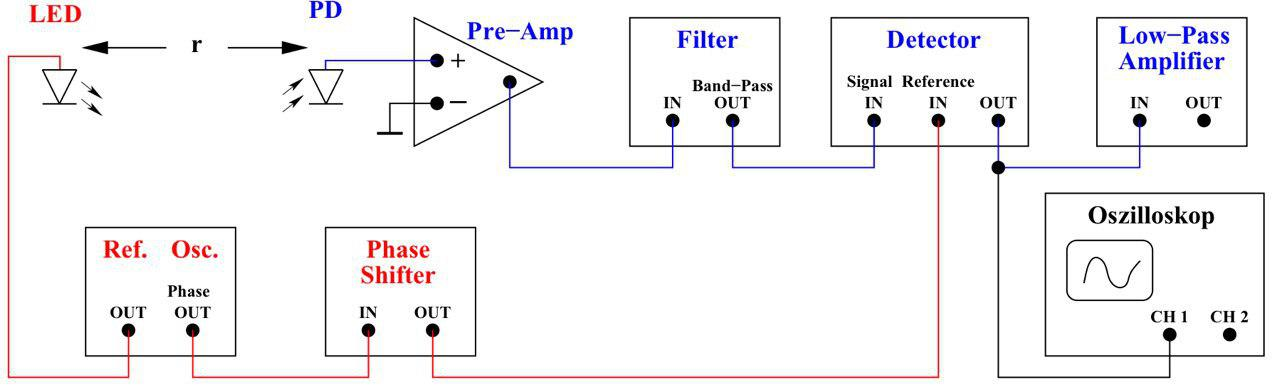
\includegraphics[width=0.7\textwidth]{bilder/LED.jpg}
    \caption{LED/Photodiodenschaltung \cite[5]{Anleitung}}
    \label{fig:LED}
\end{figure}  
\end{enumerate}